

\paragraph*{Status, 25 October 2026 (Part 2).} Sections 1--8 carry the road law $A_{\rm los}(z)=(1/\pi)\,(1-(1+z)^{-3})$ (register T-10), the distinction of equal numbers under different operators, the background adapter and the finite-redshift tests. These are the sections the ceiling runs of 24 October used, and the road is now one object with the floored reservoir on $\cosh^2\varphi=e^{ds}$ (Chapter~VIII, the section ``The $1/\pi$ ceiling as a recurring theme: results of 24 October 2026''). Section 6, the fate coefficient (T-11), is an open target that hands forward to the completed Home, which the 25 October edition gives its own chapter: Chapter~XIII (T-12, T-14).


\section{The two arcs that meet at the end of the volume}
Volume I begins with a floor and a source-induced lift. The floor supplies a reference level; the lift describes an accumulation attributed to a particular source. Chapters III--VII follow the source coordinate toward a completed boundary and ask how clocks, records, fields and thermal exchange behave there. Chapters VIII--X use the floor in a proposed cosmic inventory and in the organization of many-source systems. Chapter XI asks whether the released carrier account can become an independently testable radiation law.

The original ending joins these arcs in two ways. First, it identifies the limiting line-of-sight road accumulation with the matter fraction. Second, it proposes that a completed Home can supply a new floor through a change of informational indexing. Both are substantial ideas. Neither should be weakened by asking a numerical identity to establish a causal process that has not yet been specified.

This chapter therefore keeps the original proposals while separating four levels of statement. An identity follows from the chosen counts. A conditional theorem follows after its physical premises are declared. An adapter imports a conventional geometry or evolution law. A conjecture identifies a possible continuation whose mechanism remains to be found. The end of the volume is strongest when these levels remain visible, because they show exactly which result a future calculation would add.

The word ``fate'' also requires care. The future of a cosmological solution is a statement about evolution in proper time. The saturation of an integral along the present past light cone is a statement about progressively more distant emission events. A change of radial distance convention is yet another operation. The three can be related by a theory, but they cannot be interchanged by notation.

\section{The road law and what it actually proves}
For the nonnegative redshift domain of the original proposal, define
\begin{equation}
 A_{\rm los}(z)=A_0R\left[1-(1+z)^{-\widehat d}\right]
 =\frac1\pi\left[1-(1+z)^{-3}\right],\qquad z\geq0.
 \label{c12:road}
\end{equation}
The model uses $A_0R=1/\pi$ and $\widehat d=3$. Direct differentiation gives
\begin{equation}
 \frac{dA_{\rm los}}{dz}=\frac3\pi(1+z)^{-4}>0,
 \qquad
 \frac{d^2A_{\rm los}}{dz^2}=-\frac{12}\pi(1+z)^{-5}<0.
 \label{c12:roadderivatives}
\end{equation}
Thus the road starts at zero, initially rises with slope $3/\pi$, is monotone and concave, and has the exact limit $1/\pi$. Its survival factor is
\begin{equation}
 f(z)=1-A_{\rm los}(z)=1-\frac1\pi+\frac1{\pi(1+z)^3}.
 \label{c12:survival}
\end{equation}
For $z\geq0$, $1-1/\pi<f(z)\leq1$. No dynamics is needed to prove these statements. They are properties of the proposed function, not yet a derivation of that function from microscopic transport.

At small redshift the expansions are
\begin{align}
 A_{\rm los}(z)&=\frac1\pi\left(3z-6z^2+10z^3+O(z^4)\right),
 \label{c12:roadseries}\\
 f(z)&=1-\frac{3z}{\pi}+\frac{6z^2}{\pi}+O(z^3).
 \label{c12:fseries}
\end{align}
These coefficients are more directly testable than an asymptotic number, once the road is connected to an observable. At $z=1$, for example, the proposed accumulation is $7/(8\pi)$ and the survival factor is about $0.7215$. Any interpretation that changes a measured distance by this factor has a substantial finite-redshift consequence. It cannot be defended solely by noting that its limiting value resembles a cosmological inventory fraction.

There is a useful alternative variable for the mathematical road. Let $u=\log(1+z)$. Then $A_{\rm los}=(1-e^{-3u})/\pi$ and
\begin{equation}
 \frac{dA_{\rm los}}{du}=3\left(\frac1\pi-A_{\rm los}\right).
 \label{c12:roadode}
\end{equation}
This is an exact differential representation of the supplied curve. It is not a future-time relaxation law: $u$ labels lookback redshift along a specified observation cone. Treating it as a clock would add a new identification and must be justified independently.

\section{Equal numbers, different operators}
The inventory assignment of Chapter VIII is
\begin{equation}
 \Omega_{m,*}=RA_0=\frac1\pi,\qquad
 \Omega_{\Lambda,*}=1-\Omega_{m,*}=\frac{\pi-1}{\pi}.
 \label{c12:inventory}
\end{equation}
An asterisk emphasizes that these are the clean count-assigned fractions before corrections or additional present-day components are specified. The original typed join is then
\begin{equation}
 A_{\rm los}(\infty)=\Omega_{m,*},\qquad
 f(\infty)=\Omega_{\Lambda,*}.
 \label{c12:typedjoin}
\end{equation}
The equality is exact as a consequence of the common input $RA_0$. It does not prove that the road operator measures matter density, or that its complement has negative pressure. An inventory is a weight assigned to sectors of a state. A propagation observable is an operation on a source, path, detector and calibration. Equal expectation values do not make those operations identical.

A stronger version of the join would start with a normalized preparation measure $\mu$ on actual source states and two declared observables, $\mathcal I_m$ and $\mathcal R_{\rm los}$. It would show
\begin{equation}
 \int \mathcal I_m\,d\mu=\frac1\pi,
 \qquad
 \lim_{z\to\infty}\int\mathcal R_{\rm los}(z)\,d\mu=\frac1\pi,
 \label{c12:operatorjoin}
\end{equation}
with both normalizations derived from the same preparation and no target-dependent adjustment. This is the source-measure interface identified in the closing review. It would replace a numerical coincidence within a grammar by a common physical cause.

The component accounting also has to close. If a spatially flat present-day Friedmann adapter includes a nonzero radiation density, then $1=\Omega_{r,0}+\Omega_{m,0}+\Omega_{\Lambda,0}$. Assigning both fractions in \eqref{c12:inventory} exactly while adding radiation makes their sum exceed one. One may work in a late-time approximation neglecting radiation, assign $\Omega_{\Lambda,0}=1-\Omega_{m,0}-\Omega_{r,0}$, or change the definition of the clean ledger. The choice must be explicit. A small correction is still a correction when the proposal claims exactness.

\section{The background adapter and its conditional late-time limit}
The original fate calculation adopts
\begin{equation}
 H^2(a)=H_0^2\left(\Omega_{r,0}a^{-4}
              +\Omega_{m,0}a^{-3}+\Omega_{\Lambda,0}\right),
 \label{c12:friedmann}
\end{equation}
with $a=1$ today and a consistent normalization of its coefficients. This is a flat radiation--matter--cosmological-constant adapter. It assumes the relevant conservation laws, an expanding branch, and a positive constant vacuum term. Under those assumptions, the dilution terms vanish as $a\to\infty$ and
\begin{equation}
 H_{\infty,\rm native}=H_0\sqrt{\Omega_{\Lambda,0}}.
 \label{c12:hinfinity}
\end{equation}
The conclusion is valid conditional mathematics, but it inherits the cosmological-constant behavior from the adapter. An inventory complement has not independently derived that behavior.

The approach can also be quantified. Factoring out $\Omega_{\Lambda,0}$ and expanding the square root gives
\begin{equation}
 \frac{H(a)}{H_0\sqrt{\Omega_{\Lambda,0}}}
 =1+\frac{\Omega_{m,0}}{2\Omega_{\Lambda,0}}a^{-3}
   +\frac{\Omega_{r,0}}{2\Omega_{\Lambda,0}}a^{-4}+O(a^{-6}).
 \label{c12:approach}
\end{equation}
Along the expanding branch, the limiting equation $\dot a/a=H_{\infty,\rm native}$ has exponential solutions. This establishes the late-time behavior of the stated adapter; it does not establish stability against arbitrary changes of the source theory or additional components.

For a component with equation of state $p=w(a)\rho c^2$, separate conservation would instead give
\begin{equation}
 \rho(a)=\rho(1)\exp\left[-3\int_1^a(1+w(\widetilde a))
                                      \,d\log\widetilde a\right].
 \label{c12:darkenergy}
\end{equation}
A constant density follows only when $w=-1$, or when a separately specified exchange compensates its evolution. If the Home population feeds an effective background, that exchange must appear in the continuity equations. A successful mechanism might derive it, but the number $(\pi-1)/\pi$ alone contains no pressure, transfer rate or stability information.

Measurements such as Planck's parameter inference and DESI's distance constraints are relevant comparators [XII.1, XII.2]. They do not measure a count identity directly: they constrain an evolution and observation model. Consequently, agreement of an adopted present-day density fraction with one parameter fit does not settle the cosmological future, and a model-specific tension should not be quoted without the exact data combination and likelihood assumptions.

\section{Past-cone saturation is not future-time saturation}
In an ordinary homogeneous cosmological chart, redshift relates an emission scale factor to the observer's scale factor through $1+z=a(t_o)/a(t_e)$. Keeping $t_o$ fixed while taking $z\to\infty$ sends the emission time toward the early universe. It does not send the observer to the future. If one sets $a(t_o)=1$ and mechanically substitutes $1+z=1/a$ into \eqref{c12:road}, one obtains
\begin{equation}
 A_{\rm los}=\frac1\pi(1-a^3).
 \label{c12:badextension}
\end{equation}
For $a>1$ this becomes negative and tends to minus infinity. The substitution is a useful diagnostic: the supplied past-cone function is not a nonnegative future saturation law on that domain.

A cosmological road should instead carry its arguments explicitly. One possible notation is $A_{\rm los}(t_o,t_e,\mathcal P)$, where $\mathcal P$ identifies the ray or route and the preparation of the medium. A homogeneous effective road might depend on an integral of a rate along the ray,
\begin{equation}
 A_{\rm los}=\mathcal F\!\left(\int_{t_e}^{t_o}
                        \Gamma(t,\mathcal P)\,dt\right),
 \label{c12:roadfunctional}
\end{equation}
but the rate, saturation function and conservation law must come from the model. Writing an integral does not by itself identify the microscopic carriers or show that their accumulation is positive.

The future limit also needs a family of observations. Does the observer follow a fixed comoving source, a fixed proper-distance source, a fixed emission-time surface, or the edge of an accessible region? Each family changes the relation among $t_o$, $t_e$ and distance. A single number called the ``remaining road'' is insufficient until that family and its clocks are chosen.

As a mathematical example only, a future variable $B(N)$ with $N=\log a$ could obey $dB/dN=\lambda(B_*-B)$ for $\lambda>0$. Then $B=B_*+[B(0)-B_*]e^{-\lambda N}$, so $B_*$ is an attractor. Choosing $B_*=1/\pi$ reproduces the desired limit but does not derive it. This toy equation identifies the missing tasks: derive the fixed point, the sign and magnitude of its relaxation, the physically allowed interval and the source of any dissipated energy.

\section{The fate coefficient and the meaning of an expansion rate}
The working draft uses
\begin{equation}
 D_{\rm native}=fD_{\rm readout}
 \label{c12:distancemap}
\end{equation}
and proposes multiplication of the background rate by $f_\infty$. There is one clear operational situation where that multiplication is correct. If a separately fixed velocity-like numerator obeys $v=H_{\rm native}D_{\rm native}$ and one fits the same numerator against $D_{\rm readout}$, then
\begin{equation}
 H_{\rm fit}\equiv\frac{v}{D_{\rm readout}}
              =fH_{\rm native}.
 \label{c12:fitrate}
\end{equation}
Assuming additionally that a future observing family has $f_\infty=\Omega_{\Lambda,*}$, and using the radiation-neglecting adapter, this gives the original expression
\begin{equation}
 H_{{\rm fit},\infty}=H_0\Omega_{\Lambda,*}^{3/2}
 =H_0\left(\frac{\pi-1}{\pi}\right)^{3/2}
 \simeq0.562834H_0.
 \label{c12:conditionalfate}
\end{equation}
This is a conditional distance-fit coefficient. The numerator, clock and calibration must remain fixed exactly as stipulated. At cosmological distances, recession velocity is not generally a directly measured local velocity, so the observation rule cannot be left implicit.

A fractional expansion rate behaves differently. For a comoving separation $D_{\rm native}=a\chi$ with fixed $\chi$, differentiating \eqref{c12:distancemap} using the same time coordinate yields
\begin{equation}
 \frac{\dot D_{\rm readout}}{D_{\rm readout}}
 =H_{\rm native}-\frac{\dot f}{f}.
 \label{c12:fractionalrate}
\end{equation}
If $f$ approaches a nonzero constant and $\dot f/f\to0$, this rate approaches $H_{\rm native}$, not $f_\infty H_{\rm native}$. A constant rescaling of distance cancels from a logarithmic derivative. This simple identity is essential to the final claim: the original multiplication cannot be described as a future Hubble rate without an operational definition that differs from the usual fractional expansion rate.

Changing the clock would add another factor. If $dt_{\rm readout}=g(t)dt$, then the measured fractional rate becomes $[H_{\rm native}-\dot f/f]/g$. Neither $g$ nor its asymptote follows from a distance fraction. Chapter IV's local invariant light speed is compatible with many coordinate or readout conventions; it does not select one of them. The calibration of clocks, rulers and propagation must be supplied together.

\begin{figure*}[t]
\centering
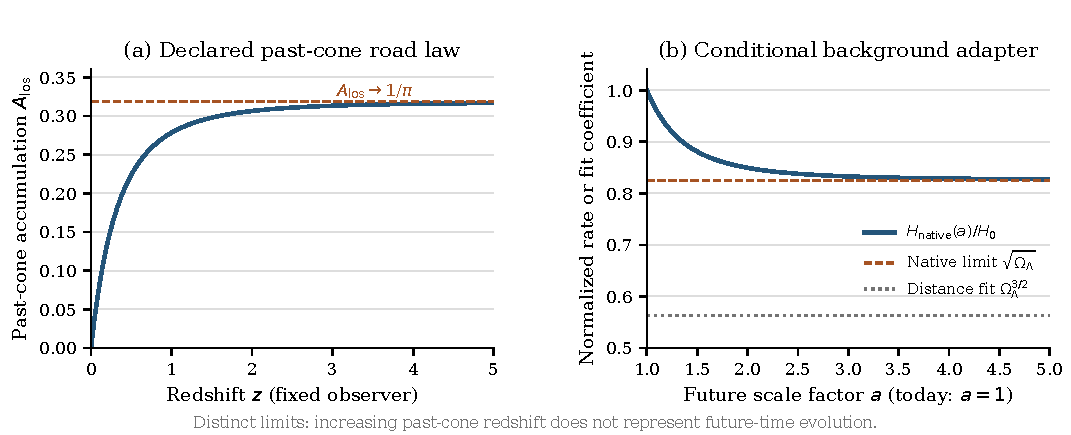
\includegraphics[width=\textwidth]{figures/ch12_distinct_limits.pdf}
\caption{Two mathematically distinct limits. (a) The declared past-cone road law $A_{\rm los}(z)=\pi^{-1}[1-(1+z)^{-3}]$ approaches $1/\pi$ as redshift increases for a fixed observer. (b) With radiation neglected, $\Omega_m=1/\pi$ and $\Omega_\Lambda=1-1/\pi$, the adopted flat matter--constant-vacuum adapter gives $H_{\rm native}(a)/H_0=\sqrt{\Omega_m a^{-3}+\Omega_\Lambda}$ and tends to $\sqrt{\Omega_\Lambda}$. The lower dotted reference, $\Omega_\Lambda^{3/2}$, is a conditional distance-fit coefficient, not the native fractional-expansion limit; it requires the additional future observing-family and calibration assumptions in the text. Past-cone saturation does not derive a future road limit. These curves are analytic illustrations of declared premises, not observational data or an independently derived SAM future.}
\label{fig:c12:limits}
\end{figure*}

\section{Numerical values with an honest uncertainty ledger}
Using the original clean fractions and the frozen Chapter VIII value $H_{0,\rm SAM}=67.2504\ {\rm km\,s^{-1}\,Mpc^{-1}}$, the native adapter limit is approximately $55.525$ in the same units and the conditional fit coefficient is approximately $37.851$. The original alternatives $H_0=68.76$ and $73.04$ give conditional fit values about $38.700$ and $41.109$. These are rescalings of a selected input, not three independent confirmations of the theory.

The exact dimensionless expression is more portable than any one dimensional value. Even so, its apparent exactness does not remove uncertainty in the choice of inventory, the road interpretation or the dynamical adapter. If $F=H_0\Omega_\Lambda^{3/2}$, first-order propagation of continuous input errors gives
\begin{equation}
 \frac{\delta F}{F}=\frac{\delta H_0}{H_0}
                  +\frac32\frac{\delta\Omega_\Lambda}{\Omega_\Lambda}.
 \label{c12:errorlinear}
\end{equation}
A variance calculation must preserve the covariance of the inputs. Structural alternatives, such as a different road operator or a nonconstant dark-energy equation of state, are not captured by this linear formula. They require separate model branches.

The closing review cautions that the small propagated temperature uncertainty in the Hubble cascade is not a total theory uncertainty. This chapter adopts that caution. A conditional number may be computed to many decimal places, but the number of printed digits should not imply that discrete choices, calibration assumptions and uncomputed source corrections are known to that precision.

\section{Finite-redshift observations and distance duality}
A useful road theory must say which distances change. In a metric description with photon number conservation and null-geodesic propagation, luminosity and angular-diameter distances obey
\begin{equation}
 D_L=(1+z)^2D_A.
 \label{c12:duality}
\end{equation}
The physical assumptions behind this relation matter more than its use as a convenient identity. Distance-duality tests compare different measurement channels and can reveal an inconsistency in an assigned propagation factor [XII.3].

Suppose a proposed readout changes the two distances by factors $g_L(z)$ and $g_A(z)$ relative to a common metric adapter. Then the diagnostic ratio is
\begin{equation}
 \eta_D(z)=\frac{D_{L,\rm readout}}{(1+z)^2D_{A,\rm readout}}
          =\frac{g_L(z)}{g_A(z)}.
 \label{c12:dualityratio}
\end{equation}
If only luminosity distance is multiplied by $1/f$, then $\eta_D=1/f$. If both distances receive the same factor, the ratio remains one. Thus a road factor is not automatically a distance-duality violation, contrary to an overly broad reading of the closing review. The violation depends on the observation map. A common rescaling still affects other distance and expansion comparisons and is not automatically viable.

For a concrete differential test, assume a flat adapter with $D_C(z)=c\int_0^z dz'/H(z')$, and apply $D_{C,\rm readout}=D_C/f$. An analyst interpreting this new distance by the same integral relation would infer
\begin{equation}
 H_{\rm inferred}(z)
 =\frac{c}{d(D_C/f)/dz}
 =\frac{H(z)f(z)^2}
 {f(z)-[H(z)D_C(z)/c]f'(z)}.
 \label{c12:inferredH}
\end{equation}
This is not simply $fH$. The derivative of the road contributes. At $z=0$, $D_C=0$ and $f=1$, so this particular map preserves the local intercept $H_0$ while changing higher-order distance behavior.

The same point appears in a small-redshift expansion. If $q_0$ is the adapter deceleration parameter, $D_C=(c/H_0)[z-(1+q_0)z^2/2+O(z^3)]$. Dividing by \eqref{c12:fseries} and fitting the same form gives
\begin{equation}
 q_{0,\rm inferred}=q_0-\frac6\pi.
 \label{c12:qshift}
\end{equation}
The shift is large. It is a falsifiable consequence of this particular uncompensated distance map, not a claim that all possible SAM road operators predict it. A viable alternative must explicitly show which other calibration or geometry factors compensate it; silently canceling the factor would erase the claimed new observable.

\section{What the completed volume establishes and what it hands forward}
The road identities establish a bounded past-cone function and its equality, within the chosen count grammar, to a clean inventory fraction. The standard background adapter gives a conditional native late-time rate. The original $\Omega_\Lambda^{3/2}$ coefficient is retained with the specific distance-fit interpretation that makes its algebra valid; it is not established as the usual fractional expansion rate. The future saturation needed for that coefficient remains a separate dynamical requirement.

The Home recurrence, carried in Chapter~XIII, gives a rigorous nonnegative exterior account, a conditional radius floor and a distinction between gross output and net growth. It does not by itself establish an impenetrable surface, a complete evaporation law, a child universe or a source of dark energy. The completed boundary can become a unifying physical object only when one source-selected action supplies those operations with their energy and information costs.

That is the useful ending of Volume I. The early source, clock, field and record constructions have exposed interfaces that the cosmological and boundary proposals must now meet. Volume II's matter and unit calibration can strengthen those interfaces, but should not be invoked as an already completed proof. The program advances when each remaining connection becomes a declared calculation whose success or failure changes the theory.

\section*{Chapter references and provenance}
\begin{enumerate}[label={\textnormal{[XII.\arabic*]}}]
\item Planck Collaboration, ``Planck 2018 results. VI. Cosmological parameters,'' \emph{Astronomy \& Astrophysics} \textbf{641}, A6 (2020). \url{https://arxiv.org/abs/1807.06209}.
\item DESI Collaboration, ``DESI DR2 Results II: Measurements of Baryon Acoustic Oscillations and Cosmological Constraints'' (2025). \url{https://arxiv.org/abs/2503.14738}.
\item Euclid Collaboration, ``Euclid: Forecast constraints on the cosmic distance duality relation with complementary external probes,'' \emph{Astronomy \& Astrophysics} (2020). \url{https://doi.org/10.1051/0004-6361/202039078}. Used for the assumptions and observational formulation of distance duality, not as a new measurement in this chapter.
\item M. Mars, \emph{Introduction to General Relativity}, Erwin Schr\"odinger Institute summer-school notes (2014), discussion of Birkhoff's theorem. \url{https://homepage.univie.ac.at/piotr.chrusciel/SummerSchool2014/Marc_Mars_Introduction_to_GR_ESI.pdf}.
\end{enumerate}
Original SAM provenance: supplied Chapter XII; the Chapter VIII horizon projection; CR002 and CR003 of the thermal-ladder records; historical Home rules H000791 and H000794--H000797; and the supplied closing review. This expansion uses those records as manuscript provenance and does not claim to have independently executed their archived calculations. The distinctions between past-cone and future limits, between distance-fit and fractional rates, and between common and channel-dependent distance factors are explicit analytical clarifications in this edition.
